\documentclass[a4paper, 10pt]{article}
\usepackage{comment} % enables the use of multi-line comments (\ifx \fi) 
\usepackage{lipsum} %This package just generates Lorem Ipsum filler text. 
\usepackage{fullpage} % changes the margin
\usepackage{graphicx}
\usepackage{xcolor}
\usepackage[]{algorithm2e}
\usepackage{listings}

\begin{document}
%Header-Make sure you update this information!!!!
\noindent
\large\textbf{Middleware Project - MPI/OpenMP} \hfill \textbf{Marco Bacis} 873199 \\
Prof. Guinea \hfill \textbf{Daniele Cattaneo} 874757 \\
Prof. Mottola

\section*{Problem Statement}
The goal of the project is to develop a system to provide analytics over high velocity sensor data originating from a soccer game.
The goal of the analysis is to report and update the ball possession time for each player and team periodically during the game.
The data used comes from the DEBS2013 challenge, in which a number of wireless sensors embedded in the shoes and a ball were used during a soccer match, spanning the whole duration of the game
The main requirements is to use OpenMP and/or MPI to compute the real-time statistics.

\subsection*{Ball possession conditions}
A player is considered in possession of the ball when
\begin{itemize}
\item He is the player closest to the ball
\item He is not farther than K meters from the ball
\item Ball possession is undefined whenever the game was paused
\end{itemize}

\subsection*{Additional Informations}
\begin{itemize}
    \item Arm/shoe attached sensors sends data at 200Hz, while the ball has a 2kHz rate
    \item As found from the DEBS2013 challenge paper, the field is half the dimension of a standard soccer field (66 x 52 meters)
    \item Each player (and even the referee) has 2 sensors, one for each arm. The goalkeeper has 4 sensors (1 more for each arm)
    \item There is no sensor data during the last 2.5 minutes before the first half ends
    \item 4 balls are used during the game, but only the one inside the field is used for the possession computation
\end{itemize}

\section*{Implementation}

\subsection*{Serial Implementation}
In order to compute the ball possessions, the algorithm must divide the sensor data into a set of {\bf time-steps} based on the sensor's data rate.
After that, for each timestep the nearest player can be found and its possession time updated.
In this case, given that the slowest sensor has a 200Hz rate, the timestep-based grouping of the records is done by dividing each record's timestamp (in picoseconds) by $1 / 200 = 0.005s = 5\,000\,000\,000ps$.
This is done while loading the game records file.


The ball sensor outputs data at 2kHz, so for each timestep group there are about 10 ball records (usually more, as many ball sensors are on at the same time, even if just one ball is used).
To compute the ball possession, for each group the nearest player is found for each of the current ball's positions, and the timestep (5ms) is distributed among those distinct positions.
The metric used to get the nearest player is only the ground-based distance, as it was seen (by watching the mmatch videos and pairing them to the ball's positions) that the $z$ measures brought to errors in the possession computation, due to their inaccuracy w.r.t the $x$ and $y$ ones.
The algorithm's pseudocode is shown in Algorithm~\ref{algorithm:main_loops}.

\begin{algorithm}[h]
    \SetKwInOut{Input}{input}
    \SetKwInOut{Output}{output}

    \Input{Full game sensor records, game interruptions, K, T}
    \Output{Cumulated possession results every T seconds}
    \BlankLine
    \ForEach{$bucket$ of $T$ seconds records taken from the full game}{
        \ForEach{game step $s \in bucket$}{
            \If{game is not interrupted at time $s.timestep$}{
                $B \longleftarrow \emptyset$\;
                $P \longleftarrow \emptyset$\;
                \tcp{First loop, to gather just the balls records}
                \ForEach{record $r \in s$} {
                    \uIf{$r$ is a ball {\bf and} $r$ is inside the field}{
                        $B \longleftarrow B \cup r$\;
                    }
                    \uElseIf{$r$ is a player}{
                        $P \longleftarrow P \cup r$\;
                    }
                }
                \tcp{Second loop to compute the actual possession}
                $increment \longleftarrow 5ms / B.size$\;
                \ForEach{ball record $b \in B$}{
                    $minDist \longleftarrow INT\_MAX$\;
                    $minPlayer \longleftarrow \emptyset$\;
                    \ForEach{player record $p \in P$}{
                        $dist \longleftarrow p.x^2 + p.y^2$ \tcc*[r]{ground distance}
                        \If{$dist < minDist$}{
                            $minDist \longleftarrow dist$\;
                            $minPlayer \longleftarrow p$\;
                        }
                    }
                    \If{$minDist < K$}{
                        $possession[minPlayer] \longleftarrow increment$
                    }
                }
            }
        }
    }
    \caption{Main algorithm for ball possession computation}
    \label{algorithm:main_loops}
\end{algorithm}

\subsection*{Parallelization}

To parallelize the algorithm, OpenMP alone was used, as using a distributed system would have meant to move around the sensor records.
A first look at the running time of the serial algorithm shows that the majority of the time is passed reading the records csv file and parsing it.
This means that, even in the algorithm can be parallelized, the running time will not be affected much, and the processing time is too low to gain much advantage by transferring the workload to other systems.

Given that the file reading is sequential, the parsing has been implemented in parallel to it, by using \emph{pipelining} between two parallel sections of code (reading -> parsing).

As for the computation loop, it was split and parallelized in two parts.

The first loop is the outer (for each bucket of records in T seconds ranges), which was parallelized in a coarse-grained manner.
The \emph{parallel} pragma indicates that the loop is splitted in multiple threads, while the \emph{reduction} pragma means that for the possession aggregate variables, the accumulation is done in parallel.
Also, for the single player possession time increment, the \emph{atomic} pragma was added to prevent race conditions.

The second loop, for the possession time accumulation through buckets was extracted from the first one (before it was done inside it and along the print statements) and parallelized, by using a matrix of possessions (one element for each bucket, for each player), instead of a single, atomically-incremented vector (one element per player).

The matrix is filled by the first loop, then the accumulation is done with a loop over the time/bucket index and the single player.
Finally, the partial accumulations are printed to screen (and can be redirected to a file).
To improve this second loop performance, the \emph{simd} pragma was used.
The added pragma allows to execute the accumulation using SIMD execution of compatible CPUs, parallelizing it in a fine-grained way (over the single operations).

\section*{Results}

The application has been tested on a Intel core i5-8259U CPU (2.30GHz, 4 cores, 8 threads) machine with 8GB of DDR4 DRAM.
In total, 4 tests were performed (with 10 runs each): K=1m,T=60s and K=5m,T=1s; serial and parallel.

The results can be seen in Figure~\ref{fig:results}. It can be seen that the data reading part of the application hasn't gained much from the pipelining adopted, while the computation time was reduced considerably (from 3.24 to 1.12 seconds for the K=1,T=60 case, and similar for the other).
The overall speedup is 1.24X, with a 1.20X for the file reading/parsing and 3.26X for the computation.
The computation speedup is optimal and close to the number of physical cores (as the instruction mix of the running threads is similar, hyperthreading is not useful).


\begin{figure}[h]
\centering
    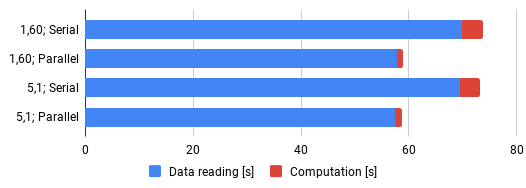
\includegraphics[width=0.66\linewidth]{images/results.png}
    \caption{Performance tests results}
   \label{fig:results}
\end{figure}



\end{document}
